

\chapter{Cronograma Detalhado}
	\label{cronograma_detalhado}
%     

\chapter{Cronograma Detalhado}
	\label{cronograma_detalhado}
%     

\chapter{Cronograma Detalhado}
	\label{cronograma_detalhado}
%     

\chapter{Cronograma Detalhado}
	\label{cronograma_detalhado}
%     \input{anexos/cronograma_detalhado}

%%%%%%%%%%%%%%%%%%%%%%% CRONOGRAMA DETALHADO

\begin{figure}[!ht]
\centering
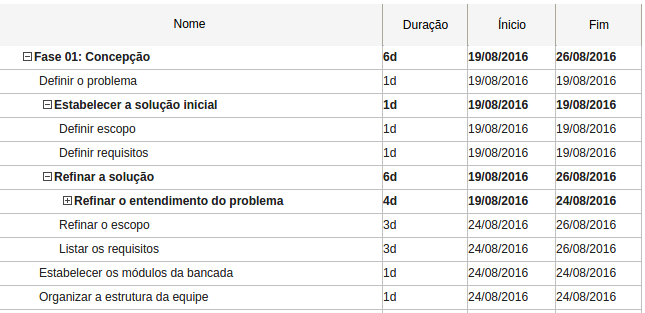
\includegraphics[scale=1]{figuras/cronograma_fase01.png}
\caption{Cronograma da Fase 01 - Concepção}
\end{figure}

\begin{figure}[!ht]
\centering
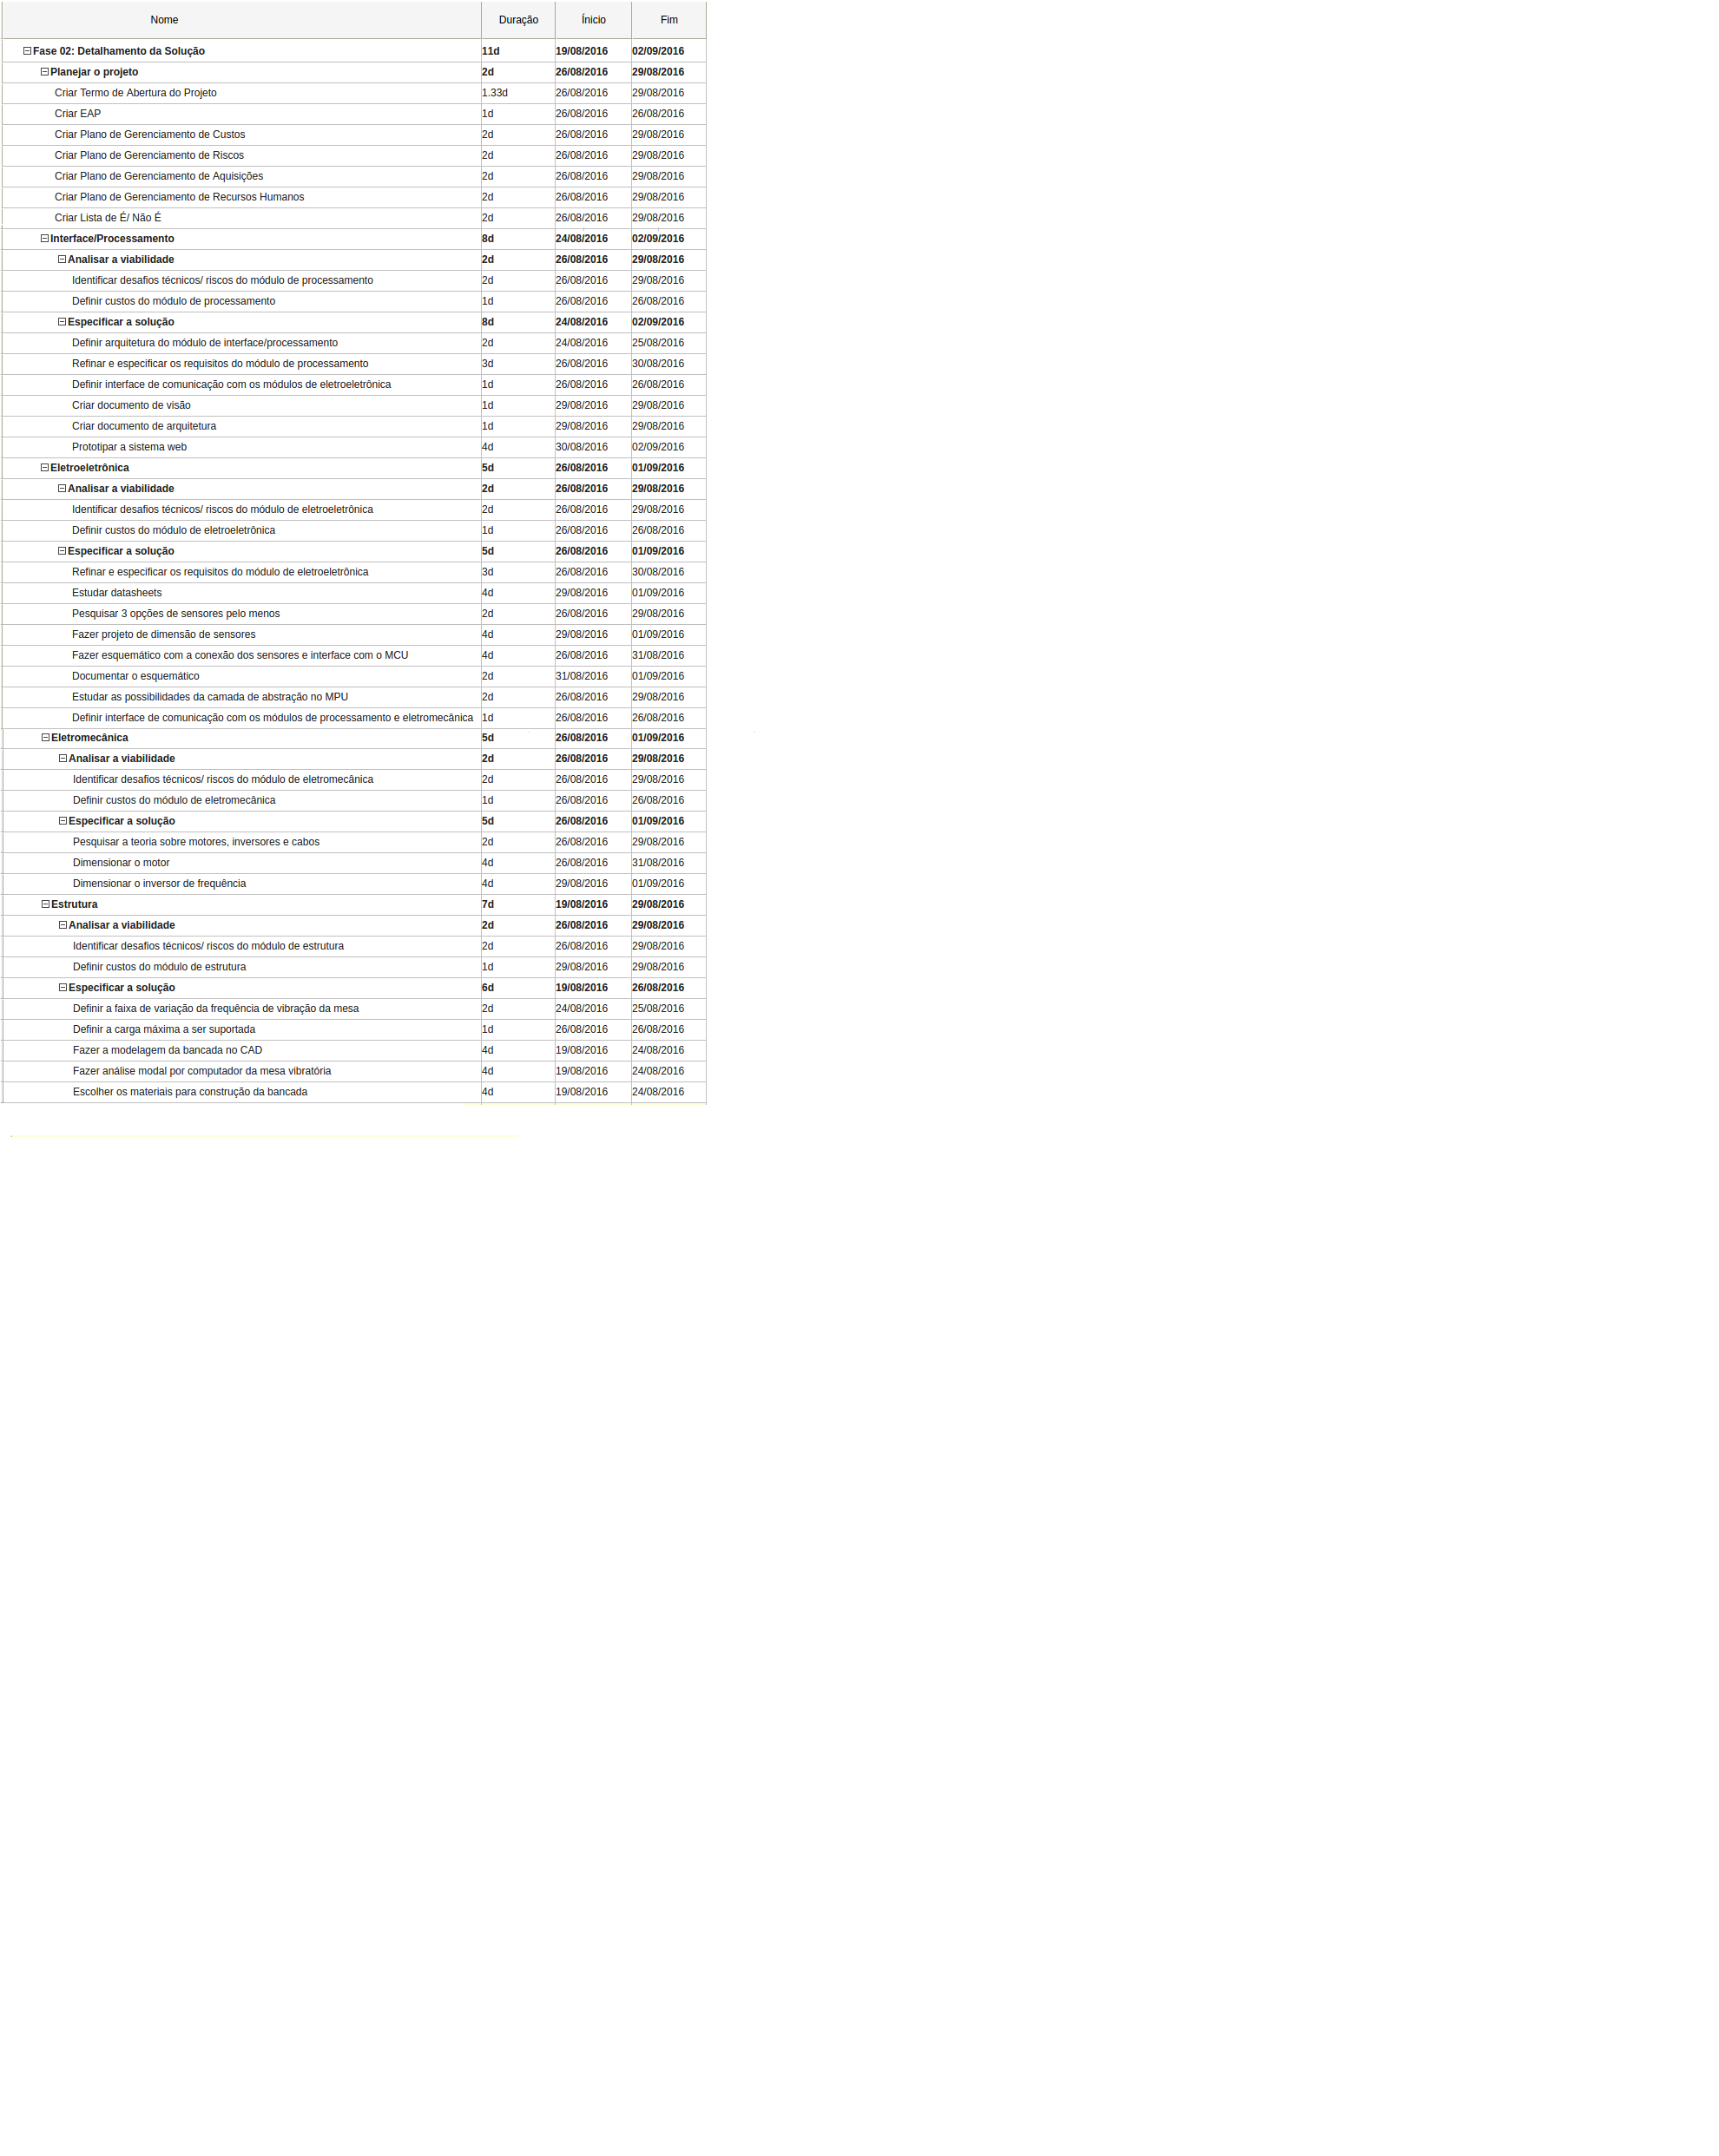
\includegraphics[scale=0.6]{figuras/cronograma_fase02.png}
\caption{Cronograma da Fase 02 - Detalhamento da Solução}
\end{figure}

\begin{figure}[!ht]
\centering
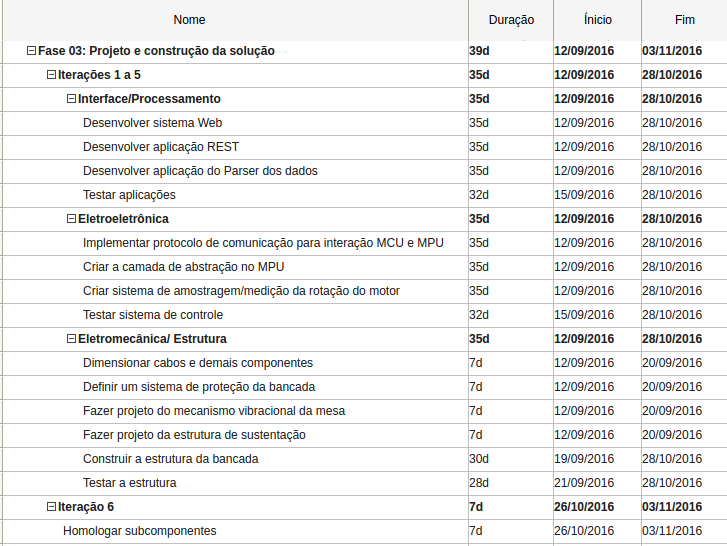
\includegraphics[scale=0.9]{figuras/cronograma_fase03.png}
\caption{Cronograma da Fase 03 - Projeto e Construção}
\end{figure}

\begin{figure}[!ht]
\centering
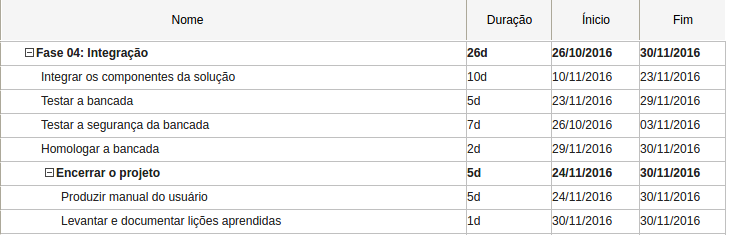
\includegraphics[scale=0.9]{figuras/cronograma_fase04.png}
\caption{Cronograma da Fase 04 - Integração}
\end{figure}
\vfill
\pagebreak

%%%%%%%%%%%%%%%%%%%%%%% FIM CRONOGRAMA DETALHADO

%%%%%%%%%%%%%%%%%%%%%%% CRONOGRAMA DETALHADO

\begin{figure}[!ht]
\centering
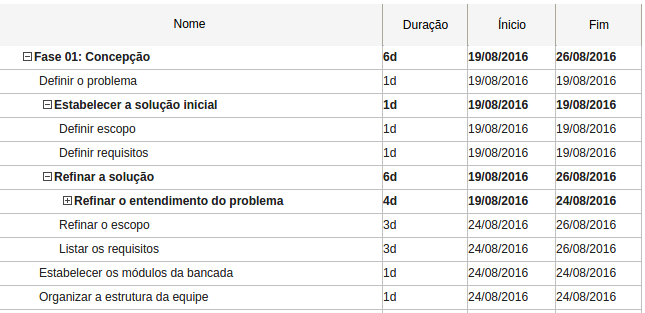
\includegraphics[scale=1]{figuras/cronograma_fase01.png}
\caption{Cronograma da Fase 01 - Concepção}
\end{figure}

\begin{figure}[!ht]
\centering
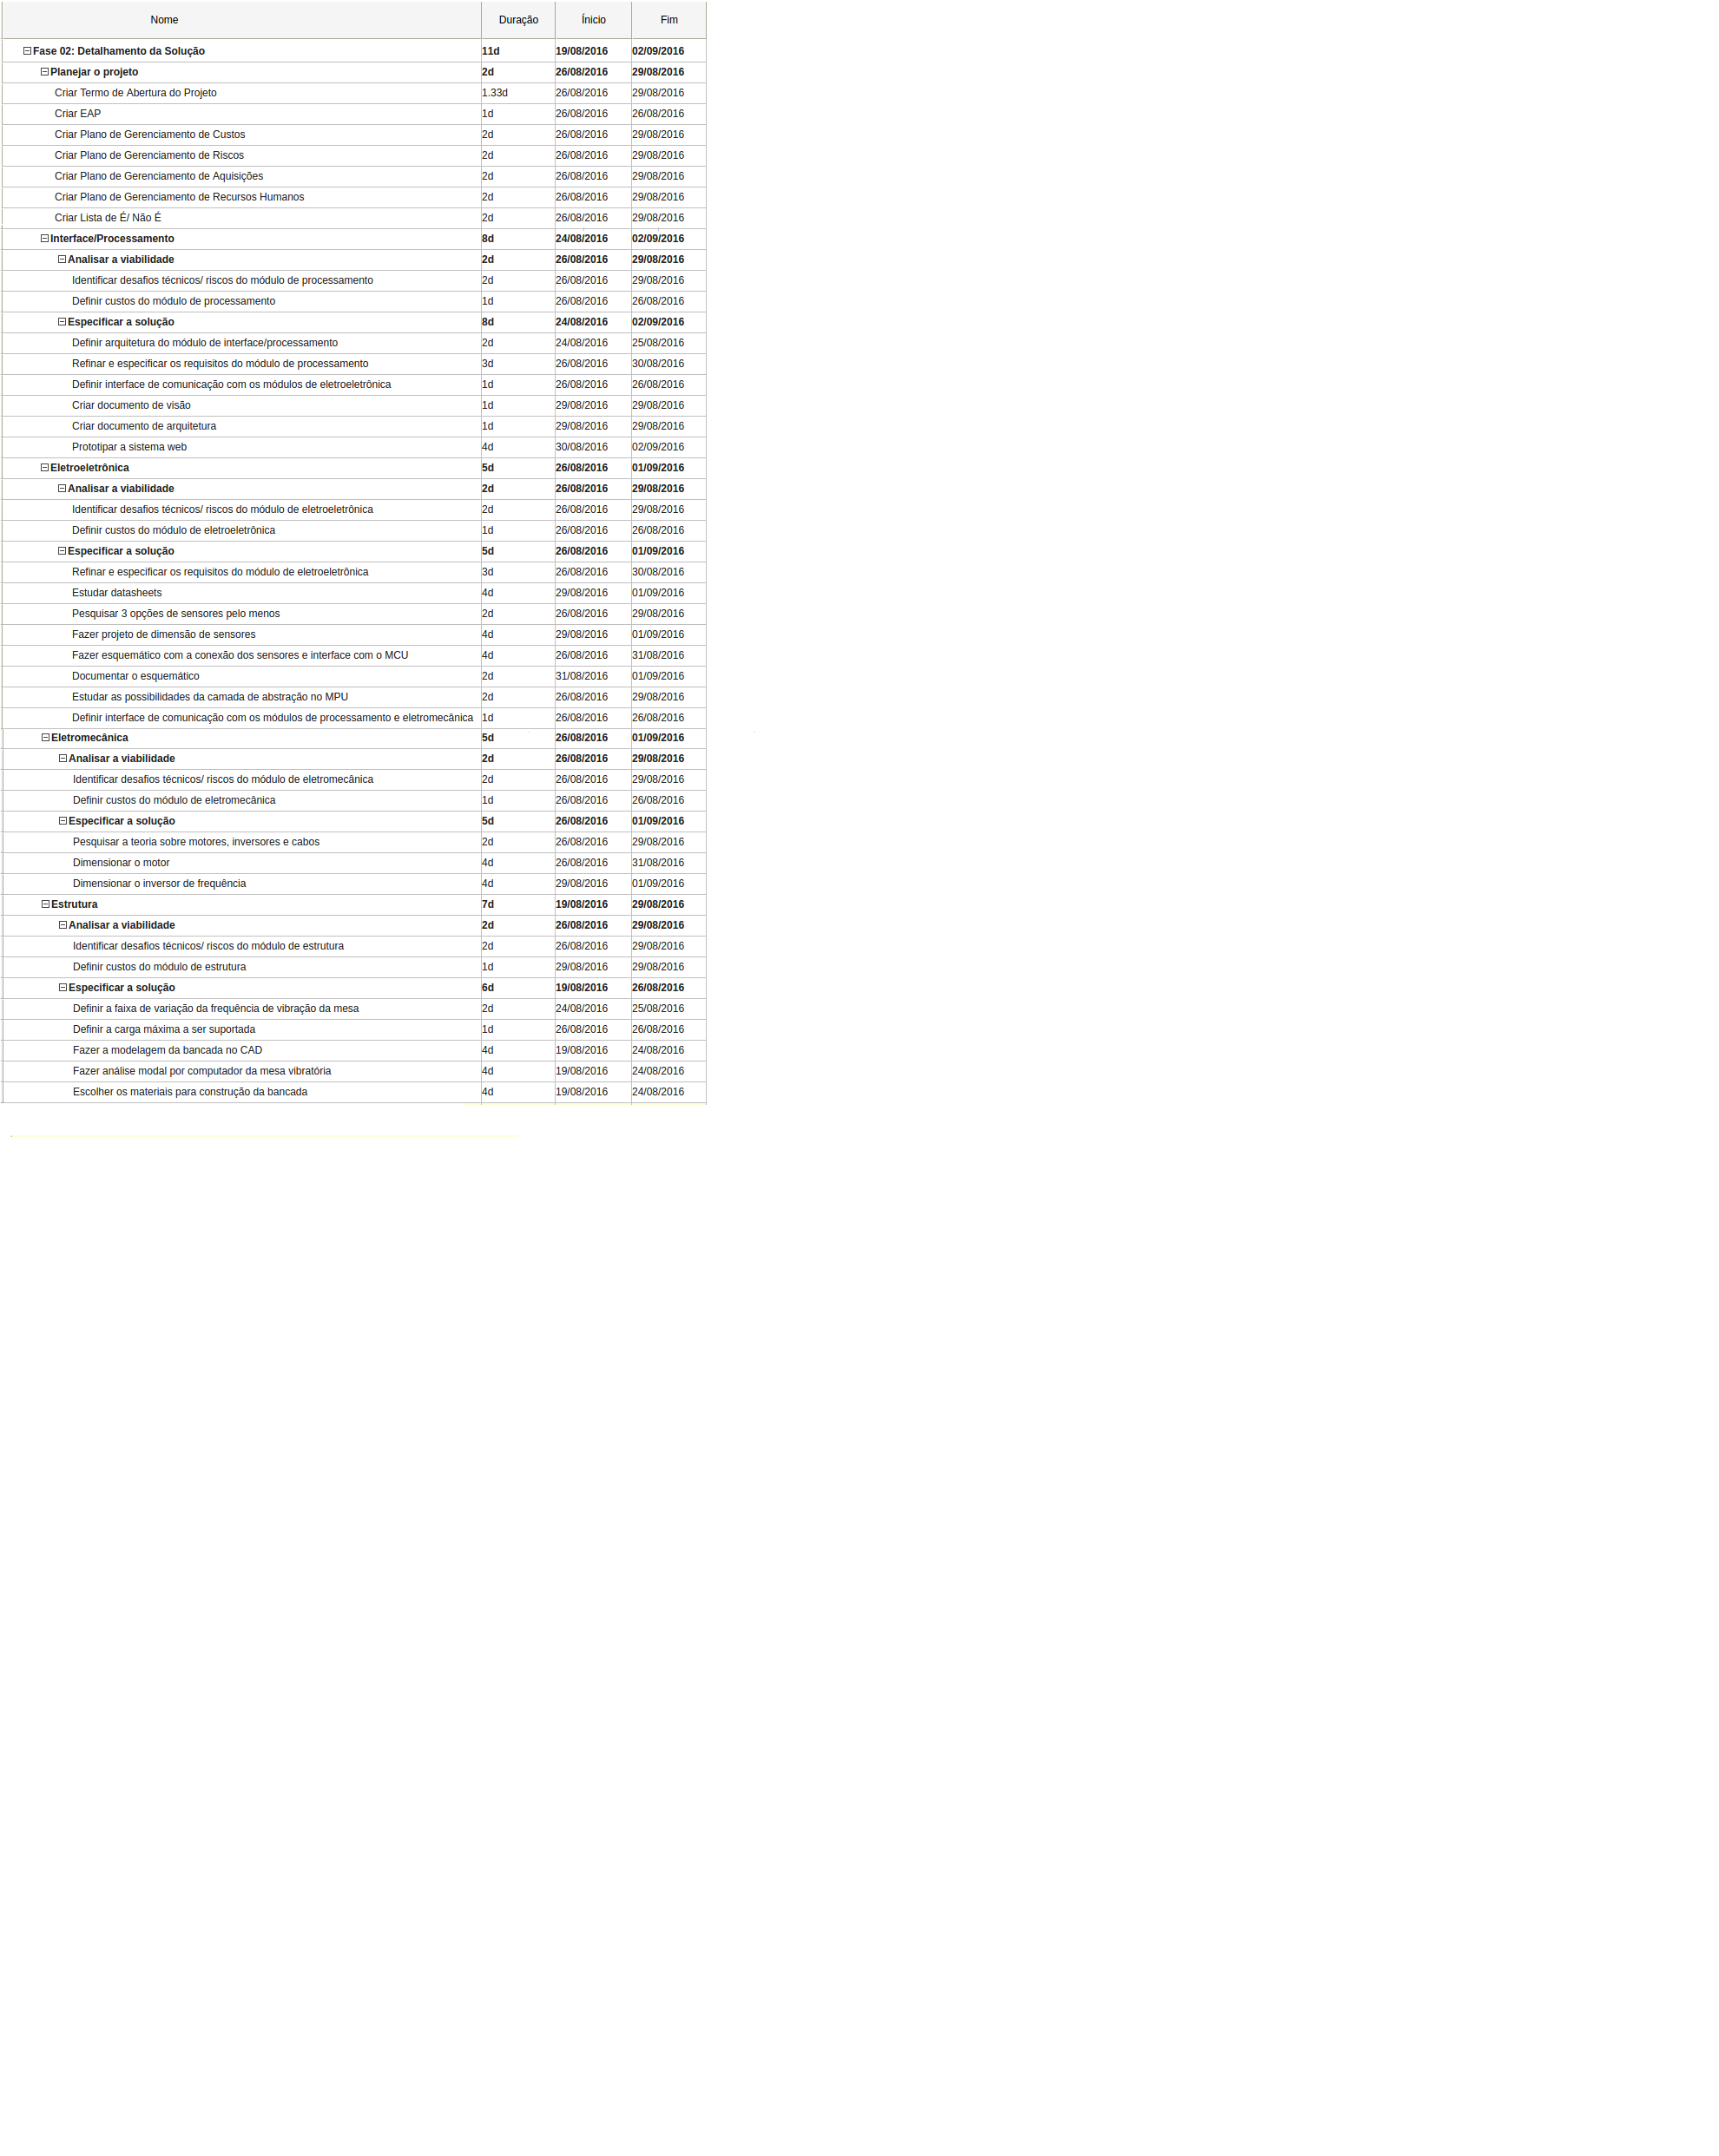
\includegraphics[scale=0.6]{figuras/cronograma_fase02.png}
\caption{Cronograma da Fase 02 - Detalhamento da Solução}
\end{figure}

\begin{figure}[!ht]
\centering
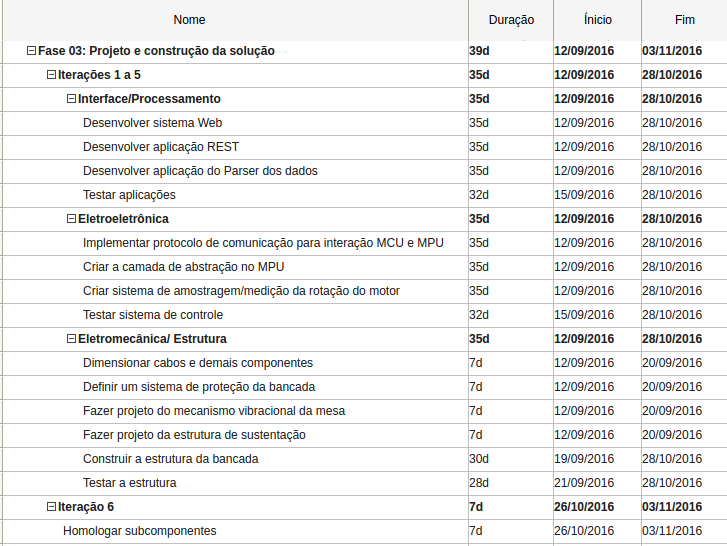
\includegraphics[scale=0.9]{figuras/cronograma_fase03.png}
\caption{Cronograma da Fase 03 - Projeto e Construção}
\end{figure}

\begin{figure}[!ht]
\centering
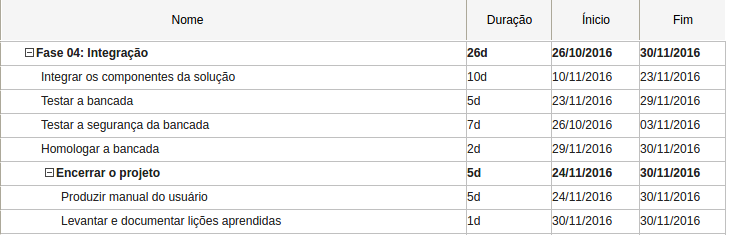
\includegraphics[scale=0.9]{figuras/cronograma_fase04.png}
\caption{Cronograma da Fase 04 - Integração}
\end{figure}
\vfill
\pagebreak

%%%%%%%%%%%%%%%%%%%%%%% FIM CRONOGRAMA DETALHADO

%%%%%%%%%%%%%%%%%%%%%%% CRONOGRAMA DETALHADO

\begin{figure}[!ht]
\centering
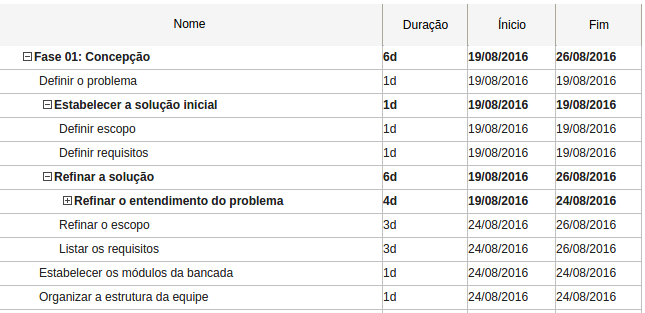
\includegraphics[scale=1]{figuras/cronograma_fase01.png}
\caption{Cronograma da Fase 01 - Concepção}
\end{figure}

\begin{figure}[!ht]
\centering
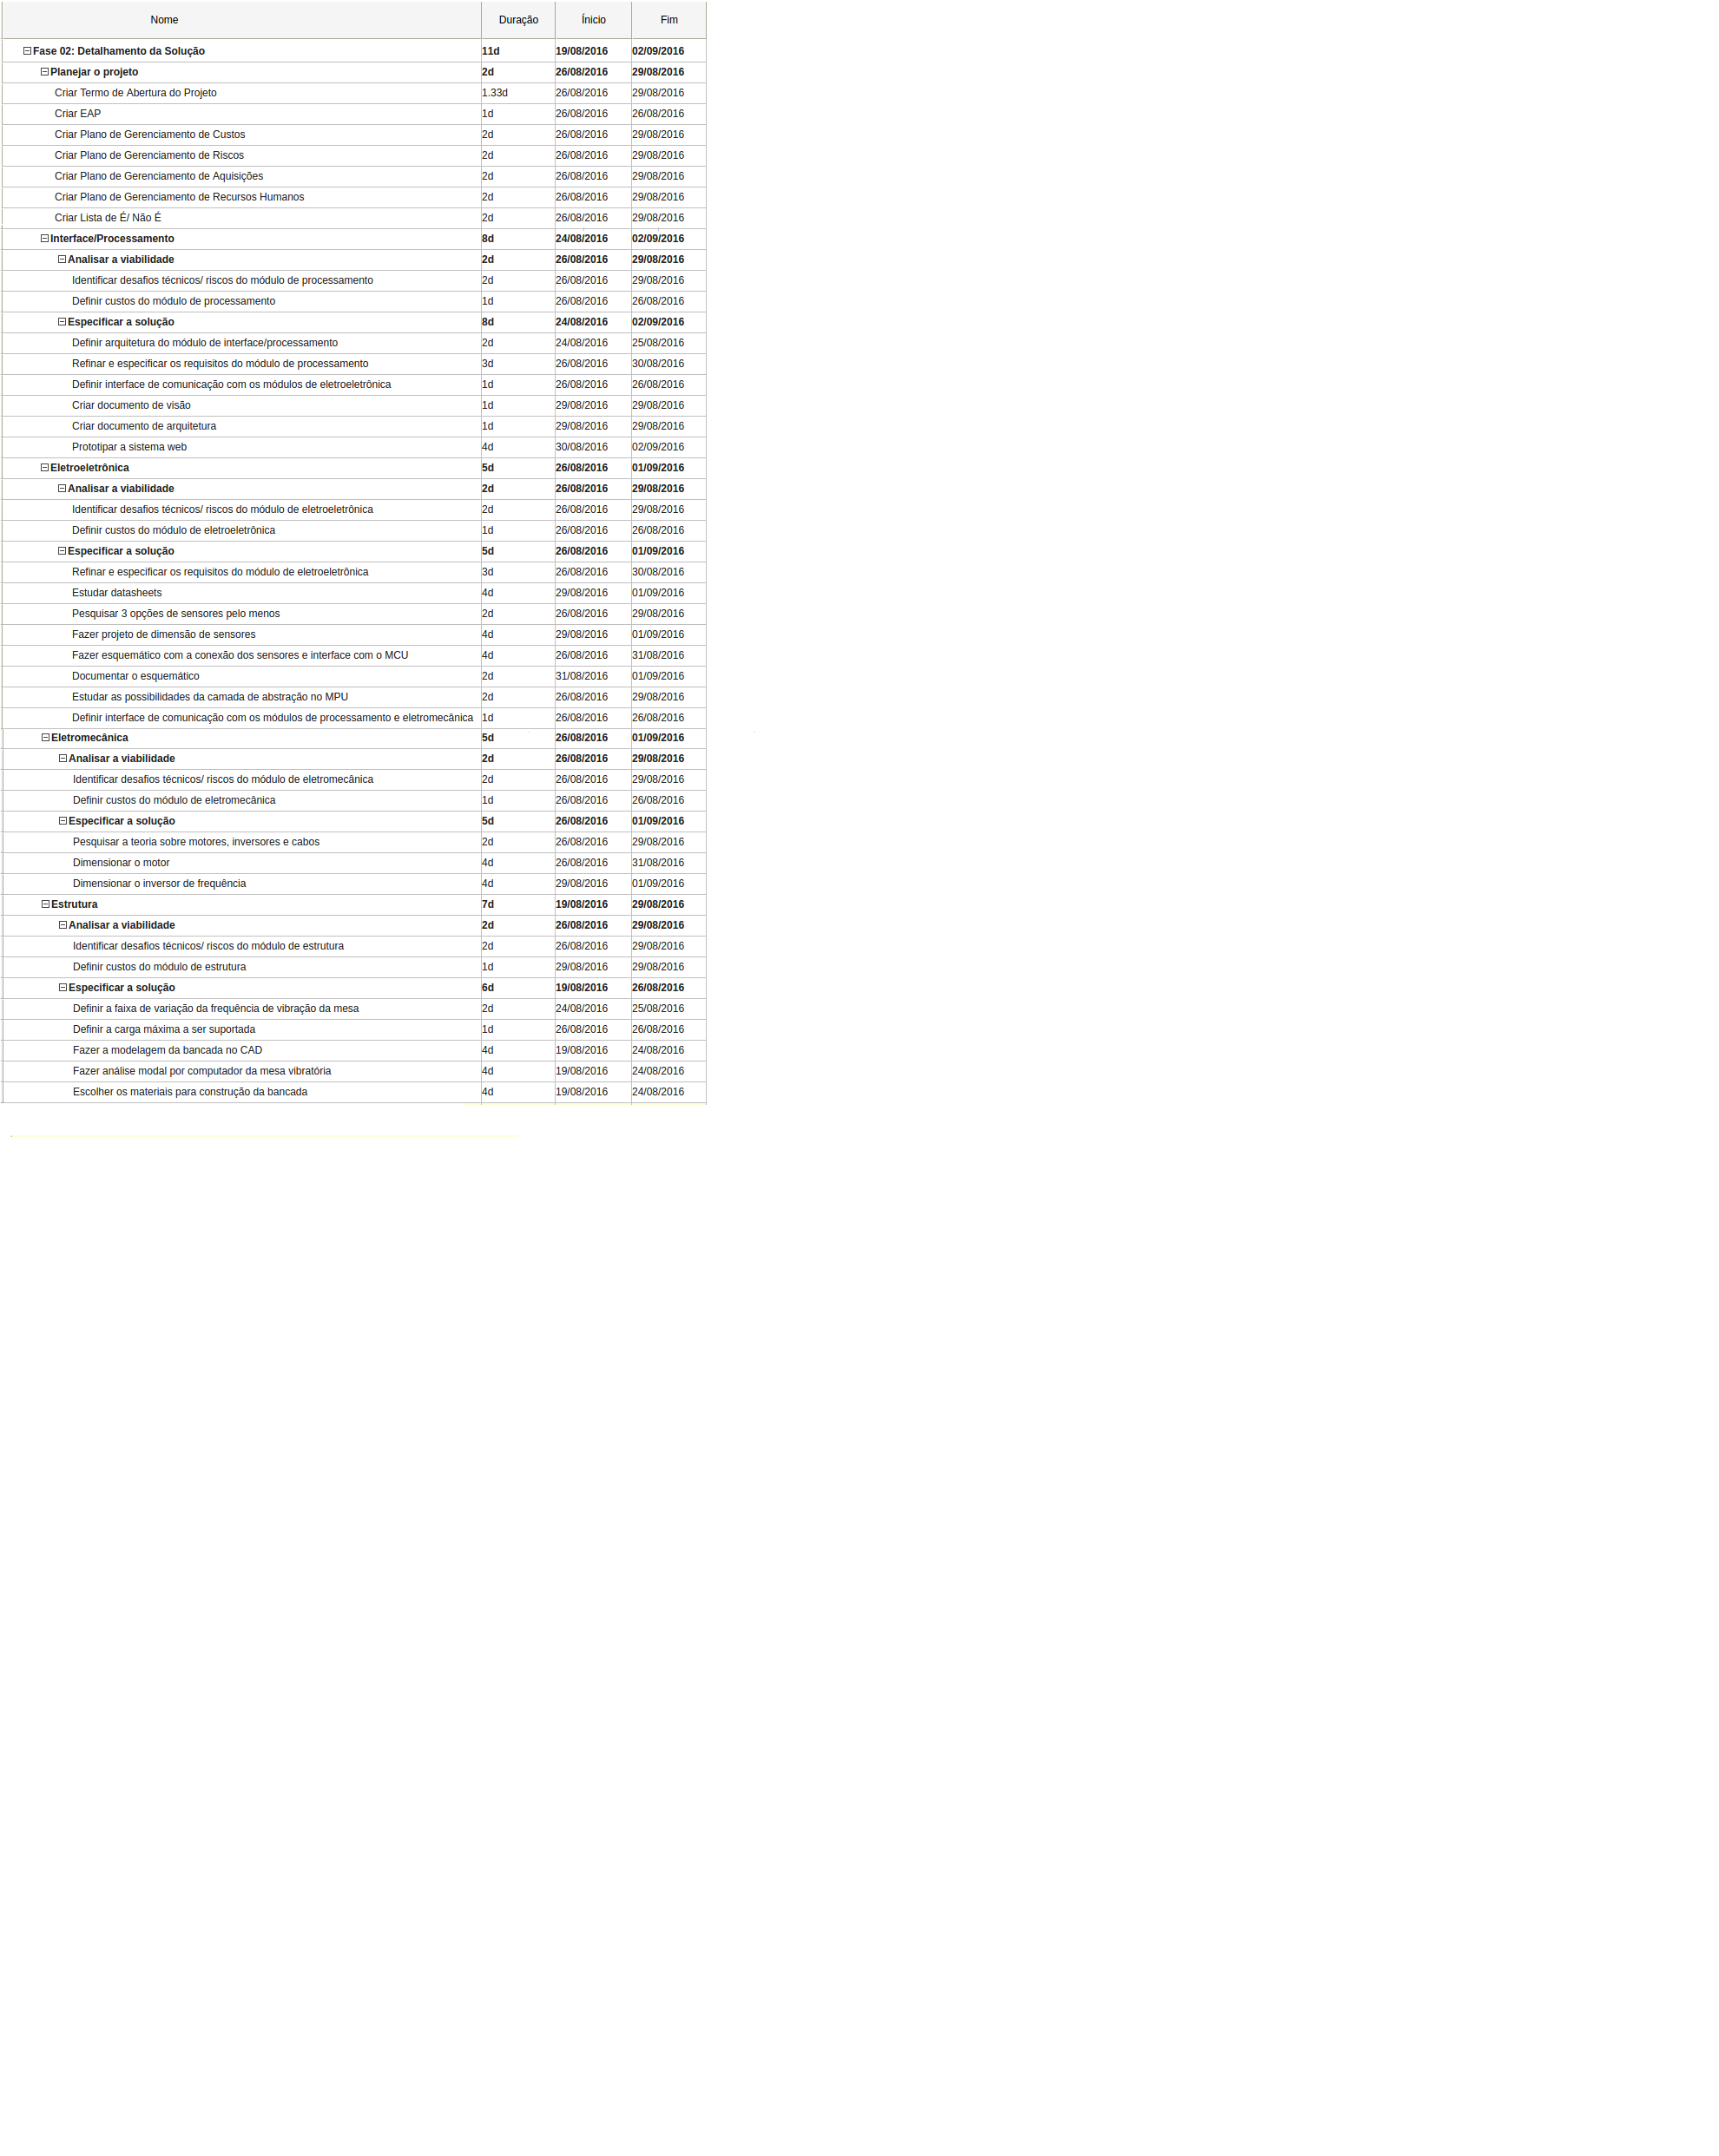
\includegraphics[scale=0.6]{figuras/cronograma_fase02.png}
\caption{Cronograma da Fase 02 - Detalhamento da Solução}
\end{figure}

\begin{figure}[!ht]
\centering
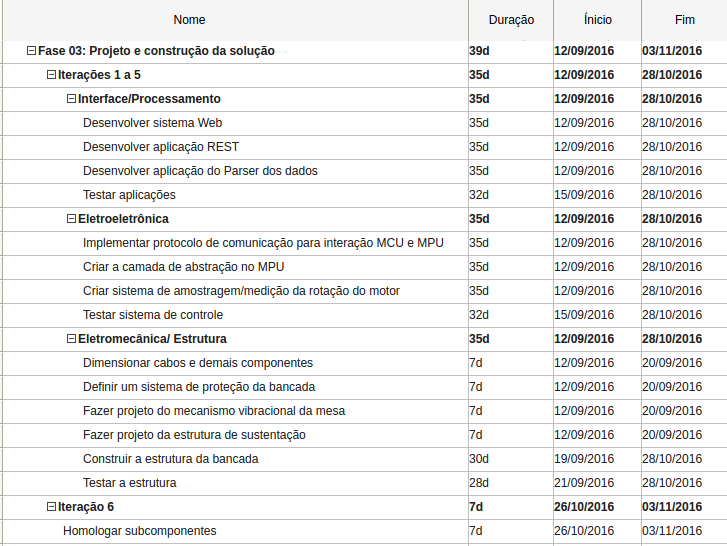
\includegraphics[scale=0.9]{figuras/cronograma_fase03.png}
\caption{Cronograma da Fase 03 - Projeto e Construção}
\end{figure}

\begin{figure}[!ht]
\centering
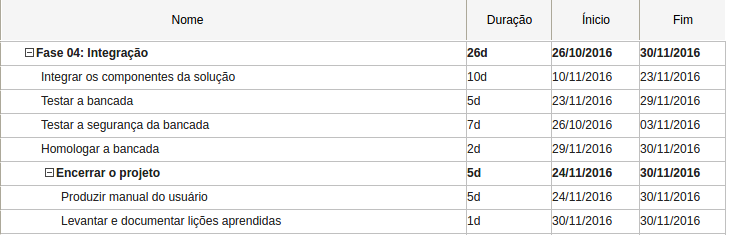
\includegraphics[scale=0.9]{figuras/cronograma_fase04.png}
\caption{Cronograma da Fase 04 - Integração}
\end{figure}
\vfill
\pagebreak

%%%%%%%%%%%%%%%%%%%%%%% FIM CRONOGRAMA DETALHADO

%%%%%%%%%%%%%%%%%%%%%%% CRONOGRAMA DETALHADO

\begin{figure}[!ht]
\centering
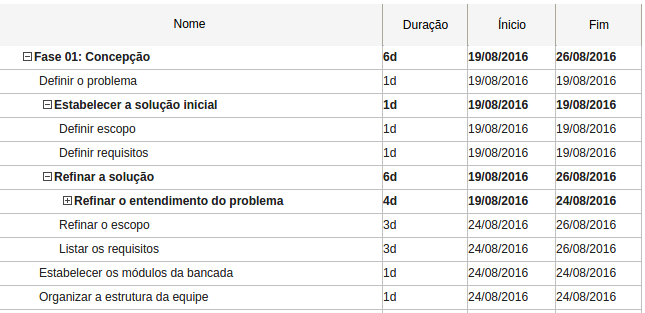
\includegraphics[scale=1]{figuras/cronograma_fase01.png}
\caption{Cronograma da Fase 01 - Concepção}
\end{figure}

\begin{figure}[!ht]
\centering
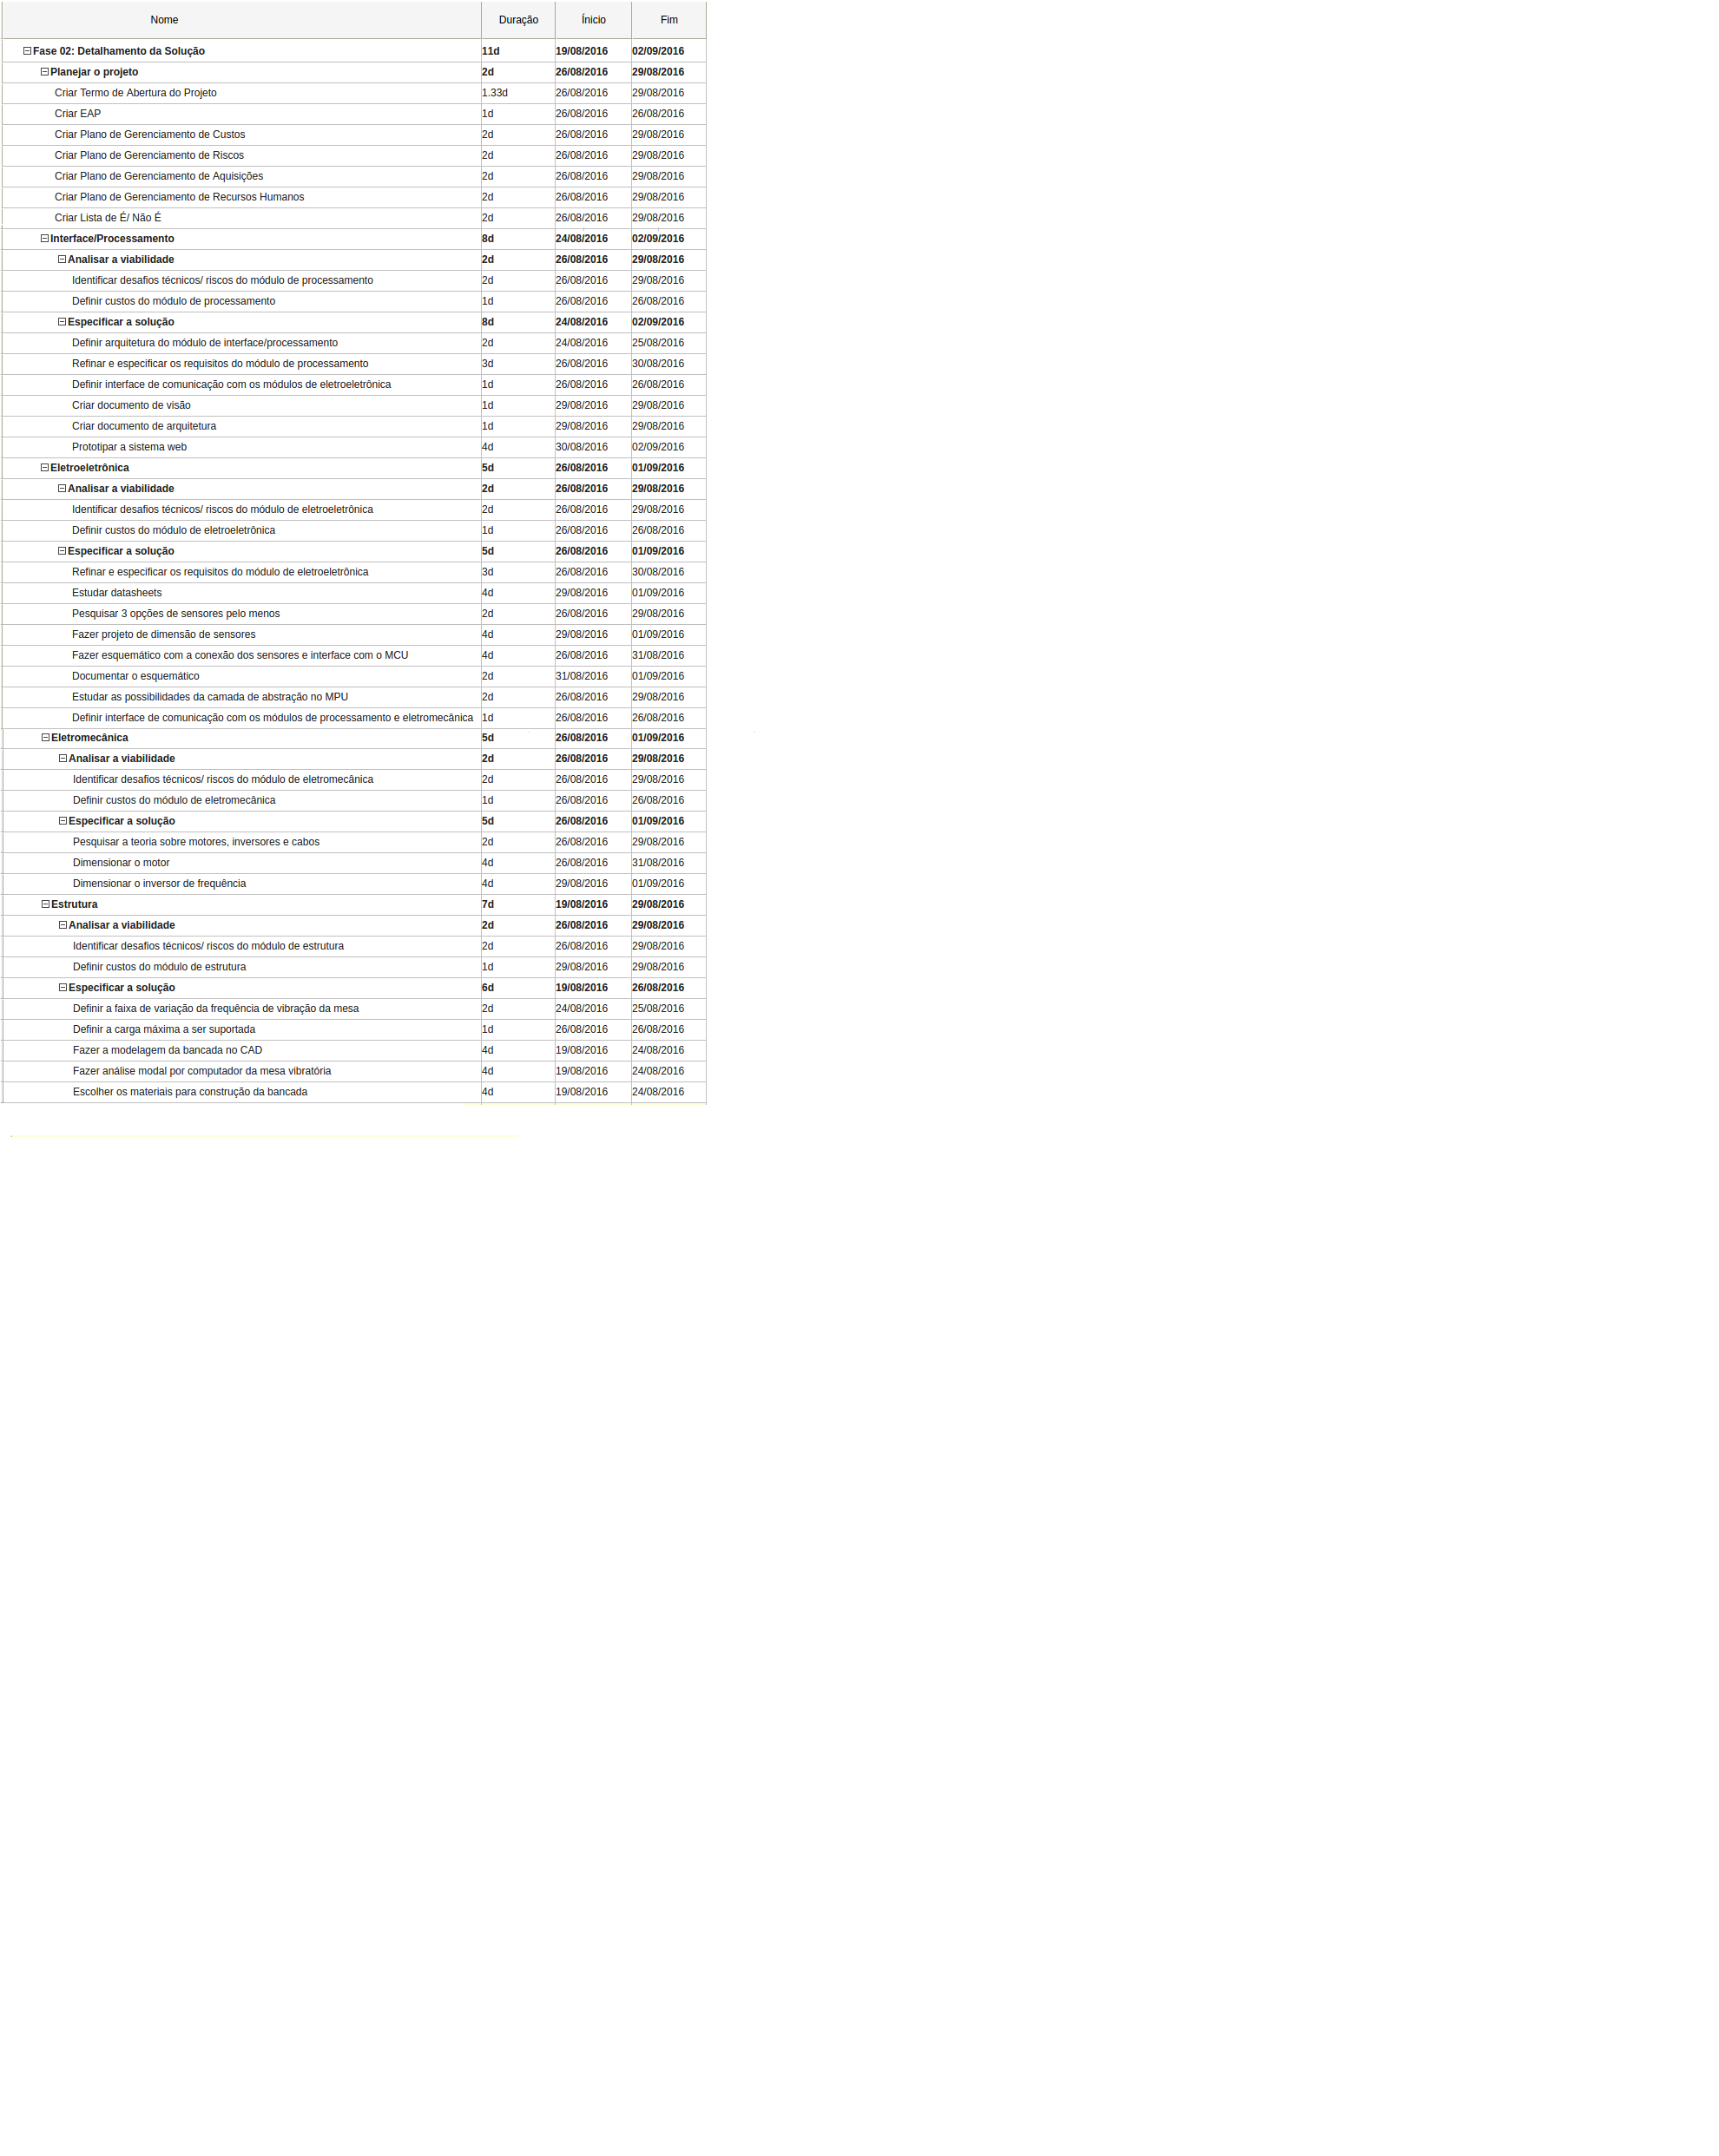
\includegraphics[scale=0.75]{figuras/cronograma_fase02.png}
\caption{Cronograma da Fase 02 - Detalhamento da Solução}
\end{figure}

\begin{figure}[!ht]
\centering
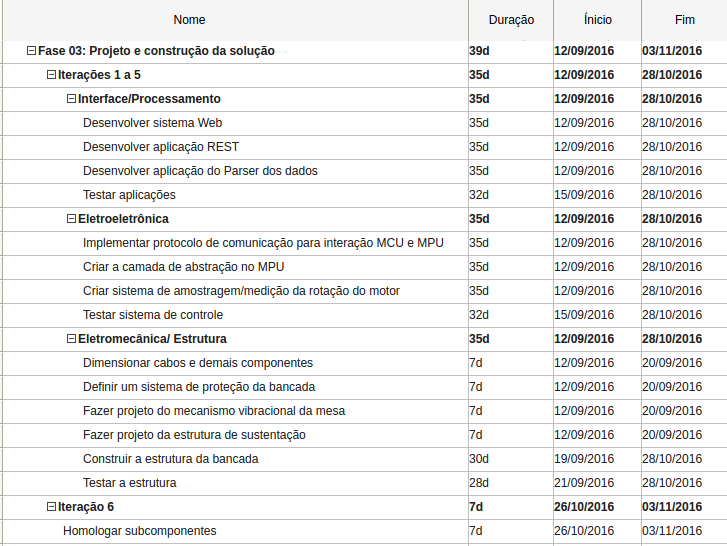
\includegraphics[scale=0.9]{figuras/cronograma_fase03.png}
\caption{Cronograma da Fase 03 - Projeto e Construção}
\end{figure}

\begin{figure}[!ht]
\centering
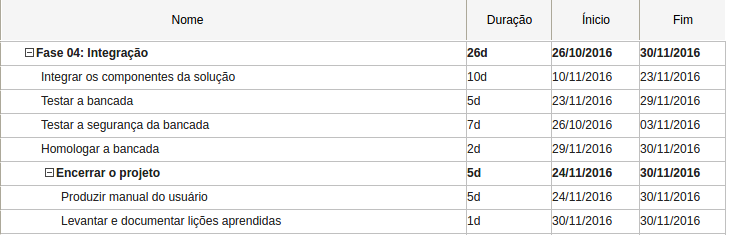
\includegraphics[scale=0.9]{figuras/cronograma_fase04.png}
\caption{Cronograma da Fase 04 - Integração}
\end{figure}

\section{Planejamento das iterações}
%%%%%%%% BACKLOGS %%%%%%%%%%%%%%555

\begin{table}[]
\centering
\caption{My caption}
%\label{my-label}
\begin{tabular}{|l|l|}
\hline
\multicolumn{1}{|c|}{\textbf{Início da Iteração}} & \multicolumn{1}{c|}{21/09}                                                                                                                            \\ \hline
\multicolumn{1}{|c|}{\textbf{Fim da Iteração}}    & \multicolumn{1}{c|}{28/09}                                                                                                                            \\ \hline
\multicolumn{1}{|c|}{\textbf{Equipe}}             & \multicolumn{1}{c|}{\textbf{Atividades planejadas}}                                                                                                   \\ \hline
\textbf{Estrutura}                                & \begin{tabular}[c]{@{}l@{}}- Definir material da mesa e espessura\\ - Estimar os pesos\\ - Fazer cálculos estruturais\end{tabular}                    \\ \hline
\textbf{Eletromecânica}                           & - Fazer sistema de acionamento do motor                                                                                                               \\ \hline
\textbf{Eletroeletrônica}                         &                                                                                                                                                       \\ \hline
\textbf{Interface/Processamento}                  & \begin{tabular}[c]{@{}l@{}}- Implementar início do experimento\\ - Implementar timer do experimento\\ - Implementar captura dos sensores\end{tabular} \\ \hline
\end{tabular}
\end{table}

\begin{table}[]
\centering
\caption{My caption}
%\label{my-label}
\begin{tabular}{|l|l|}
\hline
\multicolumn{1}{|c|}{\textbf{Início da Iteração}} & \multicolumn{1}{c|}{14/10}                                                                                                                                                           \\ \hline
\multicolumn{1}{|c|}{\textbf{Fim da Iteração}}    & \multicolumn{1}{c|}{21/10}                                                                                                                                                           \\ \hline
\multicolumn{1}{|c|}{\textbf{Equipe}}             & \multicolumn{1}{c|}{\textbf{Atividades planejadas}}                                                                                                                                  \\ \hline
\textbf{Estrutura}                                & \begin{tabular}[c]{@{}l@{}}- Comprar e instalar molas\\ - Projetar o retentor da correia\\ - Analisar o tampo com os reforços\\ - Fixar o motor\end{tabular}                         \\ \hline
\textbf{Eletromecânica}                           & \begin{tabular}[c]{@{}l@{}}- Fazer teste de integração\\ - Fazer sistema de proteção\\ - Estudar a amplitude\end{tabular}                                                            \\ \hline
\textbf{Eletroeletrônica}                         & \begin{tabular}[c]{@{}l@{}}- Testar layouts de controle do inversor\\ - Finalizar BSP\\ - Estudar obtenção da frequência * crítico\\ - Estudar viabilidade da amplitude\end{tabular} \\ \hline
\textbf{Interface/Processamento}                  & \begin{tabular}[c]{@{}l@{}}- Integrar aplicação WEB com o servidor\\ - Implementar população do banco da aplicação\\ - Implementar mais testes\end{tabular}                          \\ \hline
\end{tabular}
\end{table}


%%%%%%%%%%%%%%%%%%%%%%% FIM CRONOGRAMA DETALHADO